\documentclass[tikz,border=6pt]{standalone}
\usepackage{amsmath,amssymb}
\usepackage{xcolor}
\definecolor{accent}{HTML}{A13D2C}
\definecolor{accent2}{HTML}{2B5F6B}
\definecolor{muted}{HTML}{5A564F}
\definecolor{linecol}{HTML}{D8D2C4}
\definecolor{astroblue}{HTML}{1B4F72}
\definecolor{sunyellow}{HTML}{E8A33D}
\usetikzlibrary{calc,arrows.meta}
\usepackage{pgfplots}\pgfplotsset{compat=1.18}
\usepackage[T1]{fontenc}\usepackage{newpxtext,newpxmath}  % same fonts as the notes
\begin{document}
% Fraction of all hydrogen in level n = 2 against T, at electron pressure P_e = 20 N/m^2,
% levels 1 and 2 only in the neutral atom (rad:eq:balmer_fraction).
% x = T/(1000 K), t = x/10.  b = n_2/n_1 = 4 exp(-11.8366/t),
% R = n_p/n_1 = (kT/P_e)(2 pi m_e kT/h^2)^{3/2} e^{-13.6 eV/kT} = exp(16.6291 + 2.5 ln t - 15.7821/t),
% n_2/n_tot = b/(1 + b + R). Plotted as 10^6 n_2/n_tot.
% Peak from awk bisection: T = 9873 K, 8.738e-6.
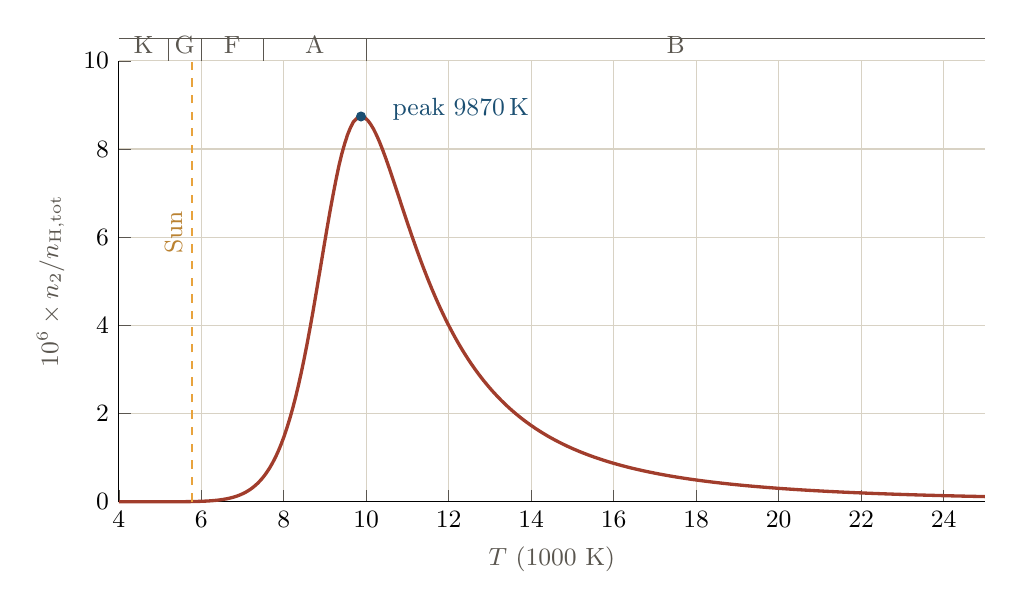
\begin{tikzpicture}[font=\small]
  \begin{axis}[width=11cm, height=5.6cm, scale only axis,
      xmin=4, xmax=25, ymin=0, ymax=10, axis lines*=left,
      xlabel={$T$ (1000 K)}, ylabel={$10^6\times n_2/n_{\rm H,tot}$},
      xtick={4,6,8,10,12,14,16,18,20,22,24}, ytick={0,2,4,6,8,10},
      tick style={muted}, every axis label/.style={font=\small, text=muted},
      grid=major, major grid style={linecol}, clip=false]
    \addplot[accent, line width=1.2pt, domain=4:25, samples=300]
      {1e6*4*exp(-118.366/x)/(1 + 4*exp(-118.366/x) + exp(16.6291 + 2.5*ln(x/10) - 157.821/x))};
    \addplot[only marks, mark=*, mark size=1.6pt, astroblue] coordinates {(9.873,8.738)};
    \node[astroblue, anchor=west] at (axis cs:10.4,8.9) {peak $9870\,\mathrm K$};
    % Sun's effective temperature
    \draw[sunyellow, dashed, line width=0.8pt] (axis cs:5.772,0) -- (axis cs:5.772,10);
    \node[sunyellow!80!black, anchor=south west, rotate=90] at (axis cs:5.772,5.4) {Sun};
    % spectral types along the top
    \pgfplotsinvokeforeach{5.2,6.0,7.5,10.0}{\draw[muted] (axis cs:#1,10) -- (axis cs:#1,10.5);}
    \node[muted] at (axis cs:4.6,10.35) {K};
    \node[muted] at (axis cs:5.6,10.35) {G};
    \node[muted] at (axis cs:6.75,10.35) {F};
    \node[muted] at (axis cs:8.75,10.35) {A};
    \node[muted] at (axis cs:17.5,10.35) {B};
    \draw[muted] (axis cs:4,10.5) -- (axis cs:25,10.5);
  \end{axis}
\end{tikzpicture}
\end{document}
